%%%%%%%%%%%%%%%%%%%%%%%%%%%%%%%%%%%%%%%%
%%%%%%%%%% TRANSPORT SUMMARY %%%%%%%%%%%
%%%%%%%%%%%%%%%%%%%%%%%%%%%%%%%%%%%%%%%%

\subsubsection{transport summary holding section}
\label{transport_summary_holding}

-- -- There are 2--3 paragraphs of info here that I have removed. They are describing a few studies that compare transport modes. I don't think that they are needed.
\cite{Kingham2013} used personal monitoring equipment and GPS devices to record individual’s exposure to traffic related pollutants of particulate matter and carbon monoxide on a number of routes in Christchurch, New Zealand. They compared the trip at the same time, day and route but by people travelling by bike (off-road) bike (on-road), car and bus during March 2009. Over 53 trips were completed. They found that cars had the highest mean CO exposure followed by bus, bike (on-road) and bike (off-road). For PM10 the pattern was similar but with much less variance. The highest was bus, followed by car, bike (on-road) and bike (off-road). PM$_{2.5}$ followed the same pattern. They concluded, at least in the city of their study, that car drivers are consistently exposed to the highest levels of carbon monoxide and ultrafine particles and that on-road cyclists are exposed to higher levels of CO PM$_{1}$ and UFP than off-road (back street) cyclists. Whether the results in this study could be generalised and applied to other cities, or even elsewhere in Christchurch, is unknown. The study did however benefit from very stable weather conditions (no rain, light wind) and Christchurch also has the advantage of suffering from little trans-boundary air pollution which could have confused the air pollution readings. Doing the same routes at the same time also improved the reliability of the study, as it meant that the results did not have to be adjusted for different background levels and/or increases in pollution from differing levels of transport at different times of the day.

\begin{figure}[H]
\centering
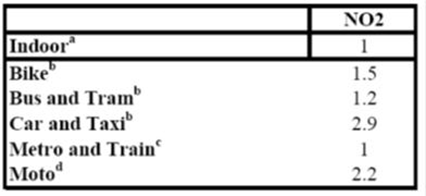
\includegraphics[scale=1]{nazelle_transport_ratios}
\caption{Transport ratios for the model from \cite{DeNazelle2013}}
\label{fig:nazelle_transport_ratios}
\end{figure}

\cite{Rojas-Rueda2013} -- A better understanding of ultrafine particle (UFP) exposure in different urban transport microenvironments is important for epidemiological exposure assessments and for policy making.
In general, smaller average particle sizes and higher UFP levels were measured at places and for travel modes in close proximity to traffic. Average trip UFP concentrations were higher in car (31,784 particles cm−³) and on bicycle (22,660 particles cm−³) compared to walking (19,481 particles cm−³) and public transportation (14,055–18,818 particles cm−³). Concentrations were highest for all travel modes during weekday morning rush hours, compared to other time periods